% !TeX root = ../main.tex
% Add the above to each chapter to make compiling the PDF easier in some editors.

\chapter{Evaluation}\label{chapter:Evaluation}
\section{Evaluation of ingredient Categorization}\label{sec:eval_cat}
As aforementioned categorisation is done with the BERT language-model provided by google and a corpus containing 8800 entries. For every new ingredient, BERT vectorizes the input and searches for a corpus-entry with the shortest distance.
The category is then copied from this entry.\\
We applied the preprocessing algorithm~\ref{section:preprocessing} before the vectorization process. We tested the impact of our preprocesser using five meals. We chose different meals out of the north/south/latin american, eurpoean and asian cuisine. In addition to that, we chose each one cocktail recipies originated in these five regions. In spite of the regional influences, we take a separate look at the cocktails, because they have more shared or similar ingredients among each other than the other recipes of the same regions. We include Cocktails to cover a wider range of ingredient categories, compared to exclusively using regular dishes. We also cover most of the daily meals by including a breakfast and a dessert for each region. Our testset also features multiple vegetarian and pescetarian dishes aswell as dishes with meat. With these attributes we hope to cover a wide range of possible ingredients, to test our programm with. Our goal was to diversify our testset as much as possible, in order to see if there is any bias within our corpus. This information would enable us to optimize our corpus efficiently. \\
\subsection{Testset}\label{sub_testset}
We will first take a detailed look at our testset. The 30 dishes include 425 different ingredients. These ingredients are divided into 25 categories. Processed by the program our testset covers: Dairy and Eggs, Spices, Fats/Oils, Poultry, Soups/Sauces, Sausages/Luncheon meats, Fruits and Fruitjuices, Pork, Vegetable, Nuts/Seeds, Beef, Beverages, Finfish/Shellfish, Legumes and Legume products, Lamb/Veal/game products, Baked Products, Sweets, Cereal Grain and pasta, Fast Food, Side Meals and Snacks. While we tried to cover a wide range of different ingredinets, we did not include ingredinets for the following categories: Breakfast cereal, Baby Food, Restaurant Foood and American Indian/alaska Native food. 
The following diagram shows how many ingredients are contained by every category. The categtories Spices(108, 25.4\%), Vegetables(72, 16.9\%) and Dairy and Egg Product(55, 12.9\%) contain the most ingredients. Figure \ref{fig:ing_dist} shows the distribution over all included categories. Figure \ref{fig:reg_dist} shows how the amount of ingredients is distributed over each region. When picking our ingredients, we searched for recipes with a larger amount of ingredients to get a larger testset. The List of recipes we used can be found in the recipe.xlsx file in the project git repository. The document also features more detailed information how many errors occured in each recipe.\\
We will now look at the result of our tests. First we will take a look at how each category performed. Followed by an analysis of each regions categorisation.
We will differentiate between correct categorisation, wrong categoriation, and not assigned. The testset will be categorized by both our implementation aswell as the initial implementation by Asela, to gain better information about the impact of our preprocesser.
 
\begin{figure}
	\centering
	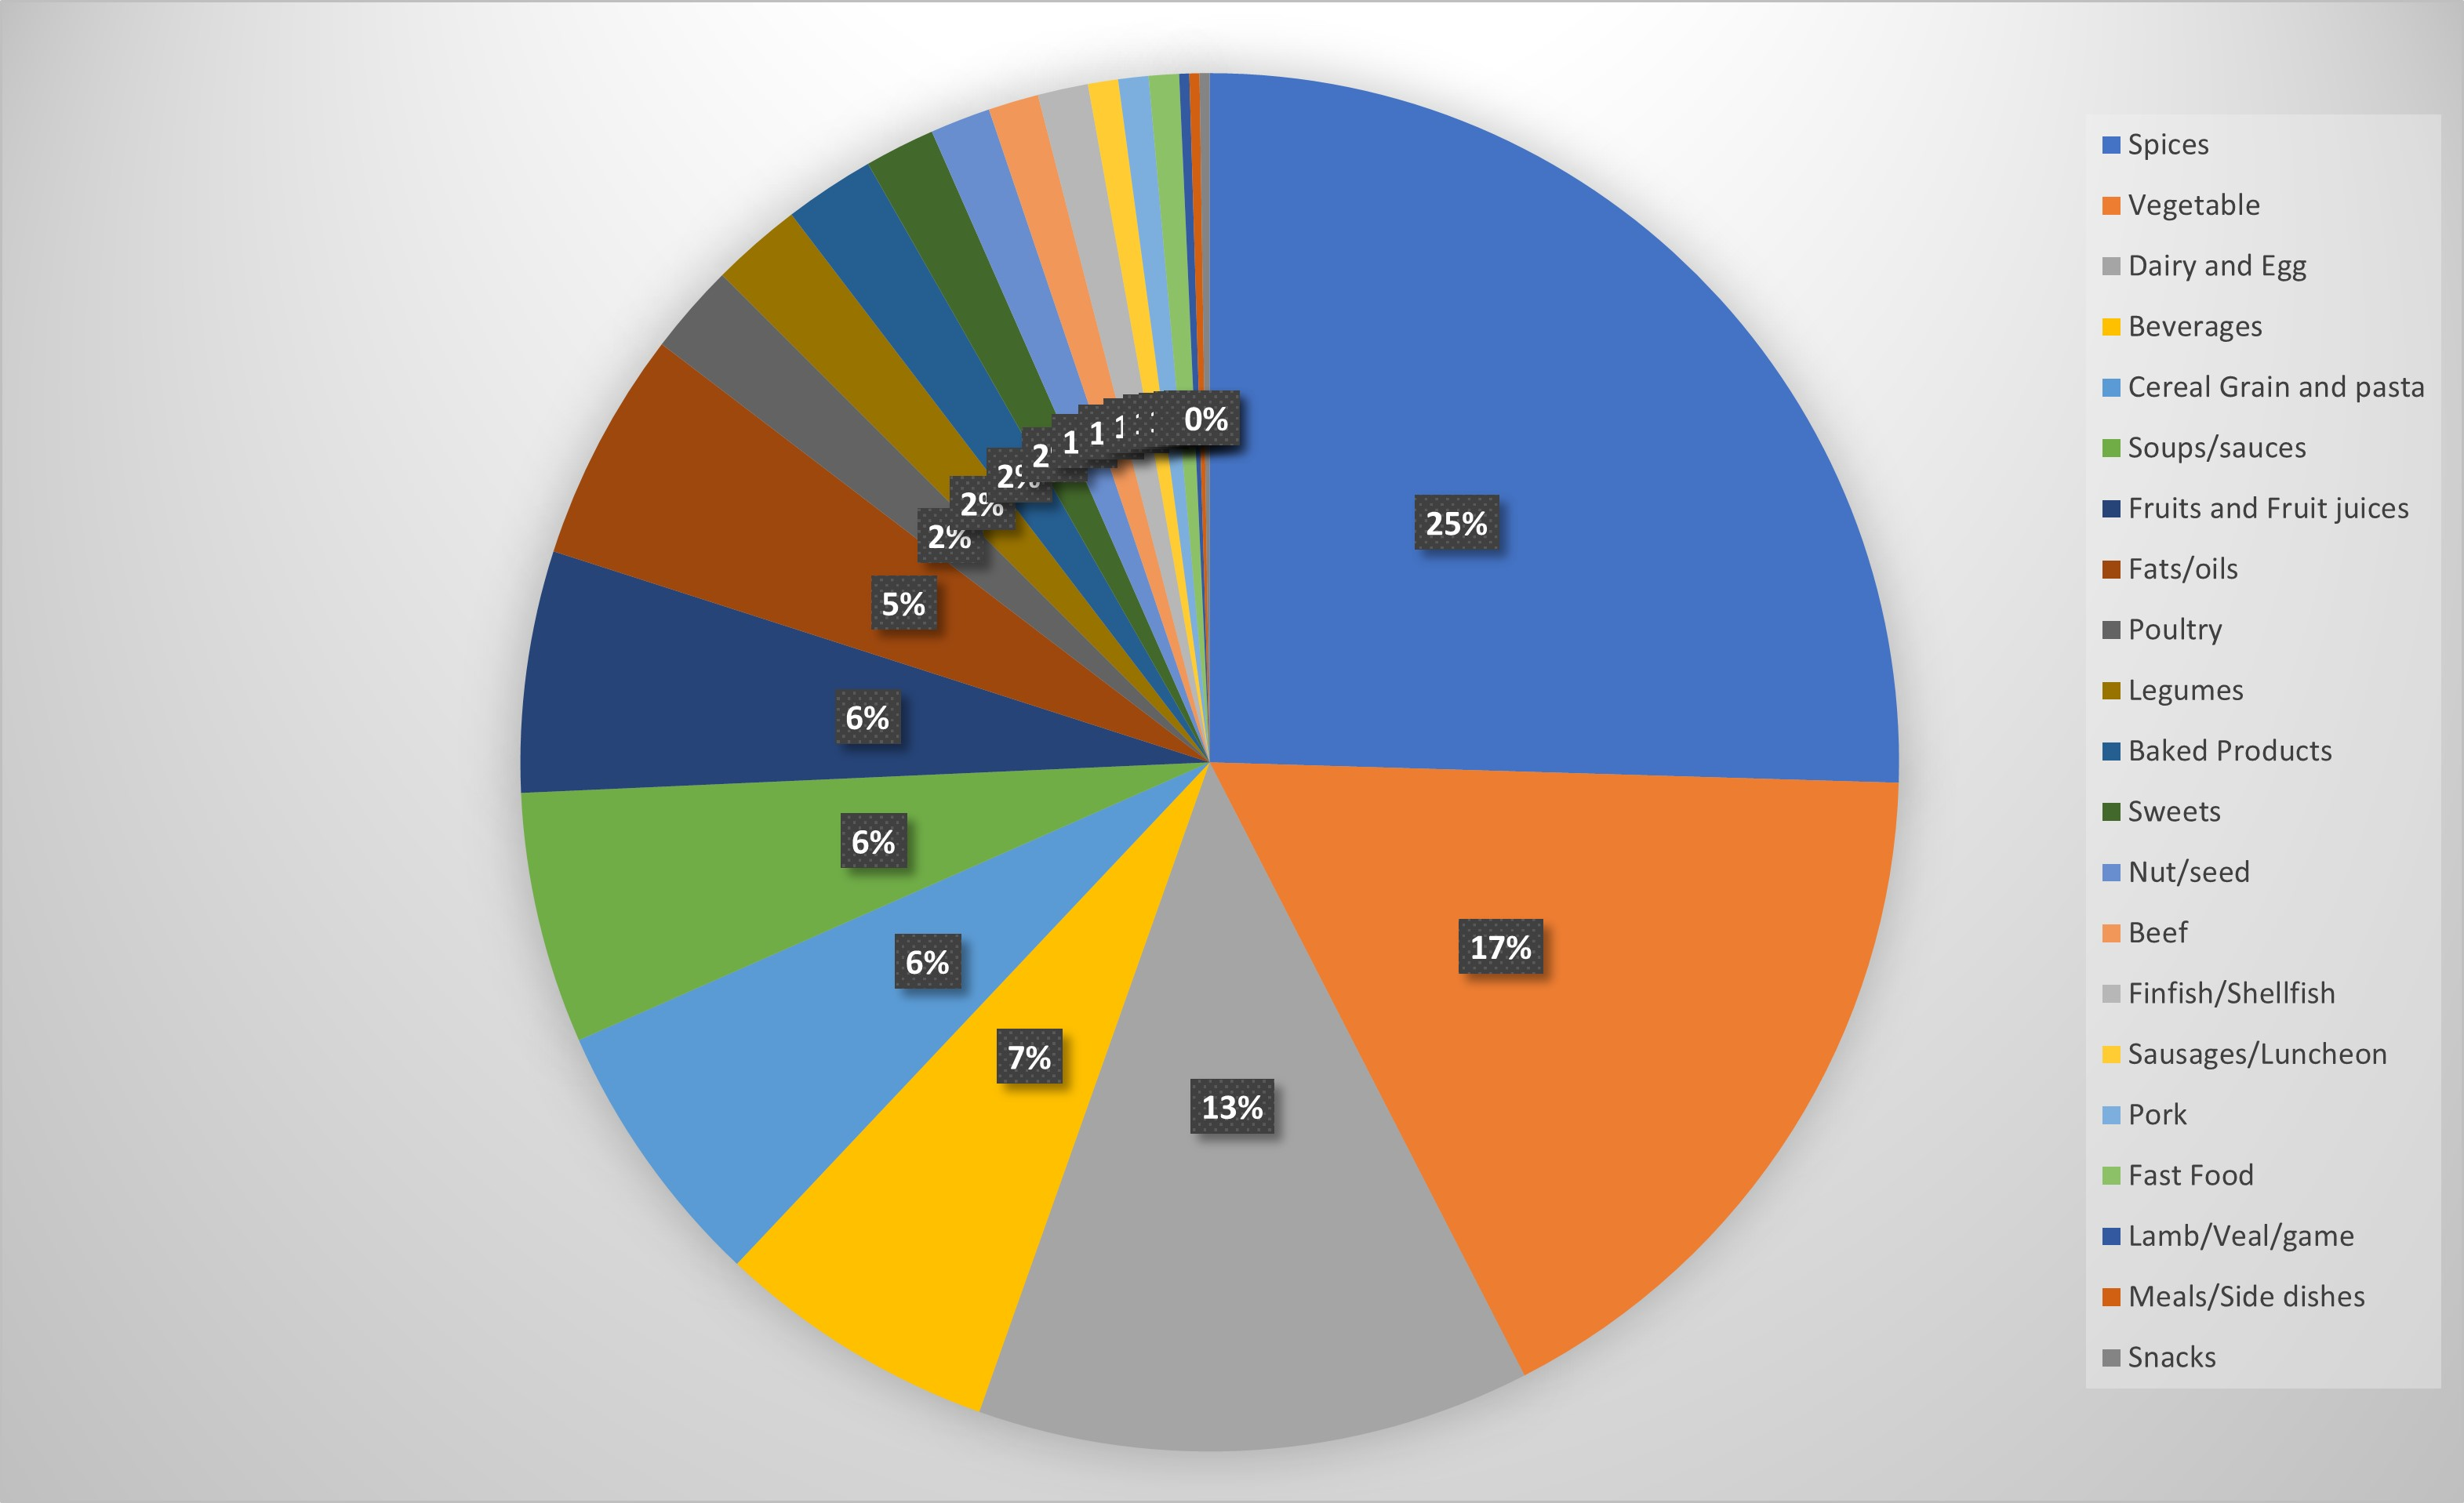
\includegraphics[scale=0.5]{Figures/ingredient_distribution.jpg}
	\caption[Ingredient Distribution]{ingredient distribution over included categories}\label{fig:ing_dist}
\end{figure}
\begin{figure}
	\centering
	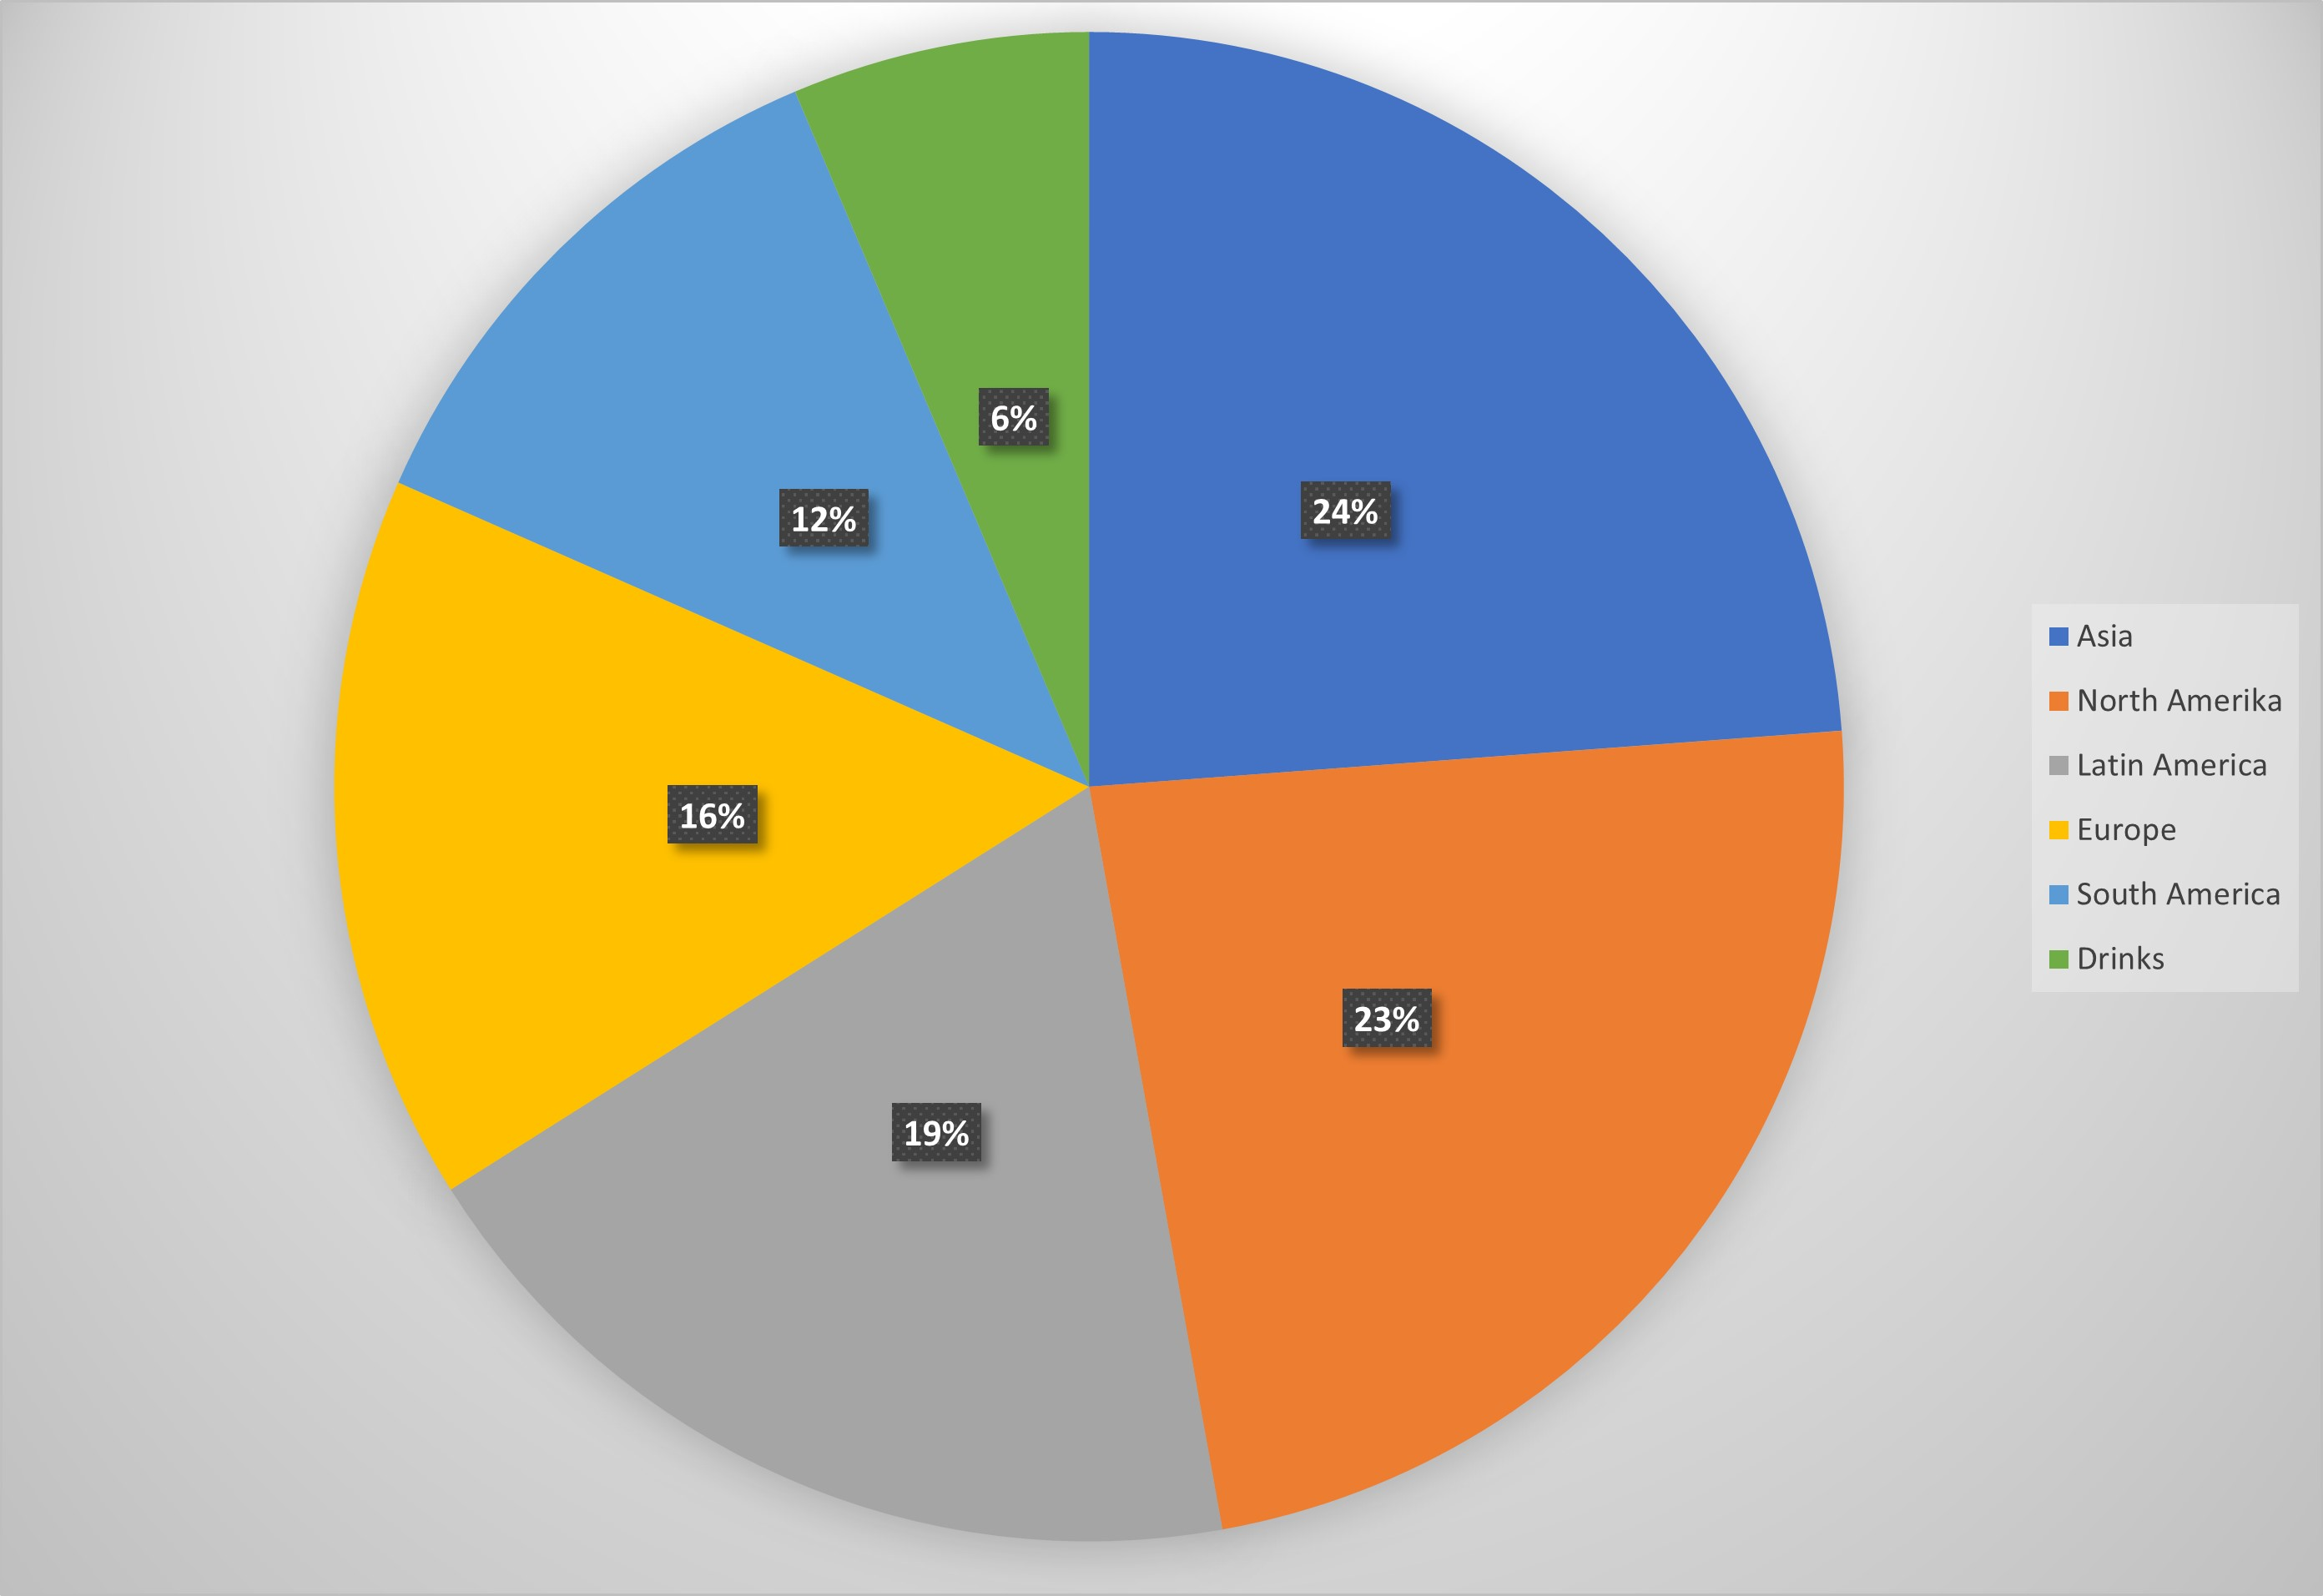
\includegraphics[scale=0.5]{Figures/region_distribution.jpg}
	\caption[Region Distribution]{ingredient distribution over regions}\label{fig:reg_dist}
\end{figure}

\subsection{Analysis of Categories}
\begin{figure}
	\centering
	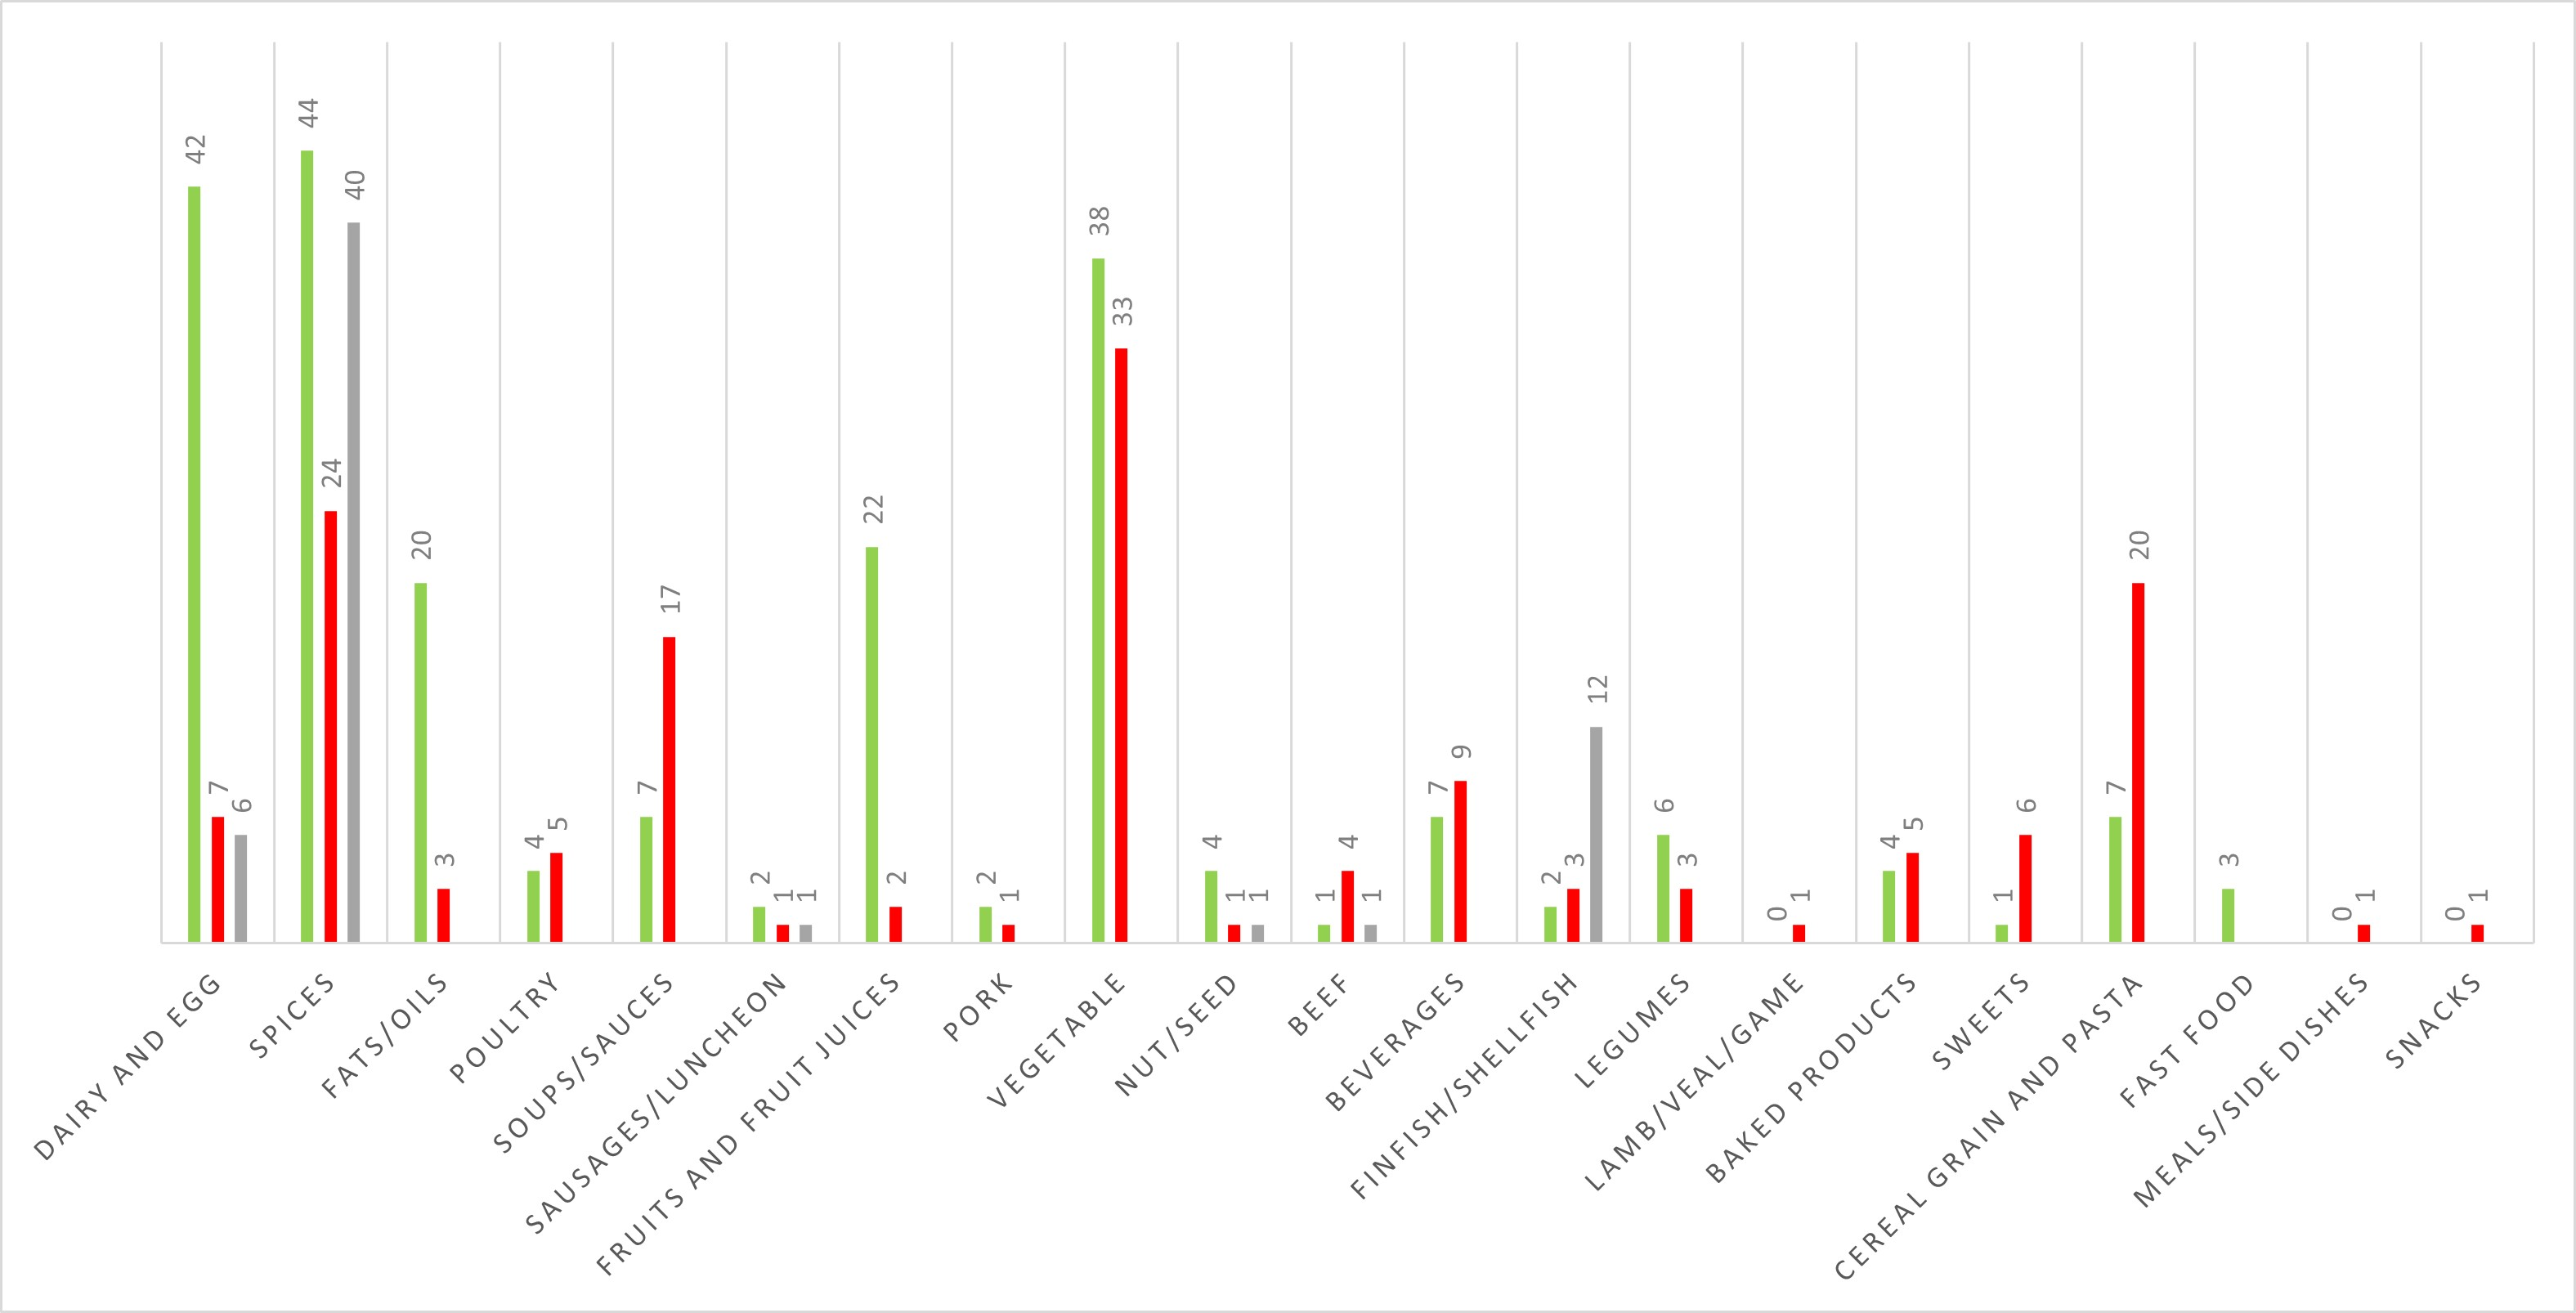
\includegraphics[scale=0.5]{Figures/categories_asela.jpg}
	\caption[Categories Analysis, initial Implementation]{Categories without preprocesser}\label{fig:cat_asela}
\end{figure}

\subsection{Analysis of Regions}
\begin{figure}
	\centering
	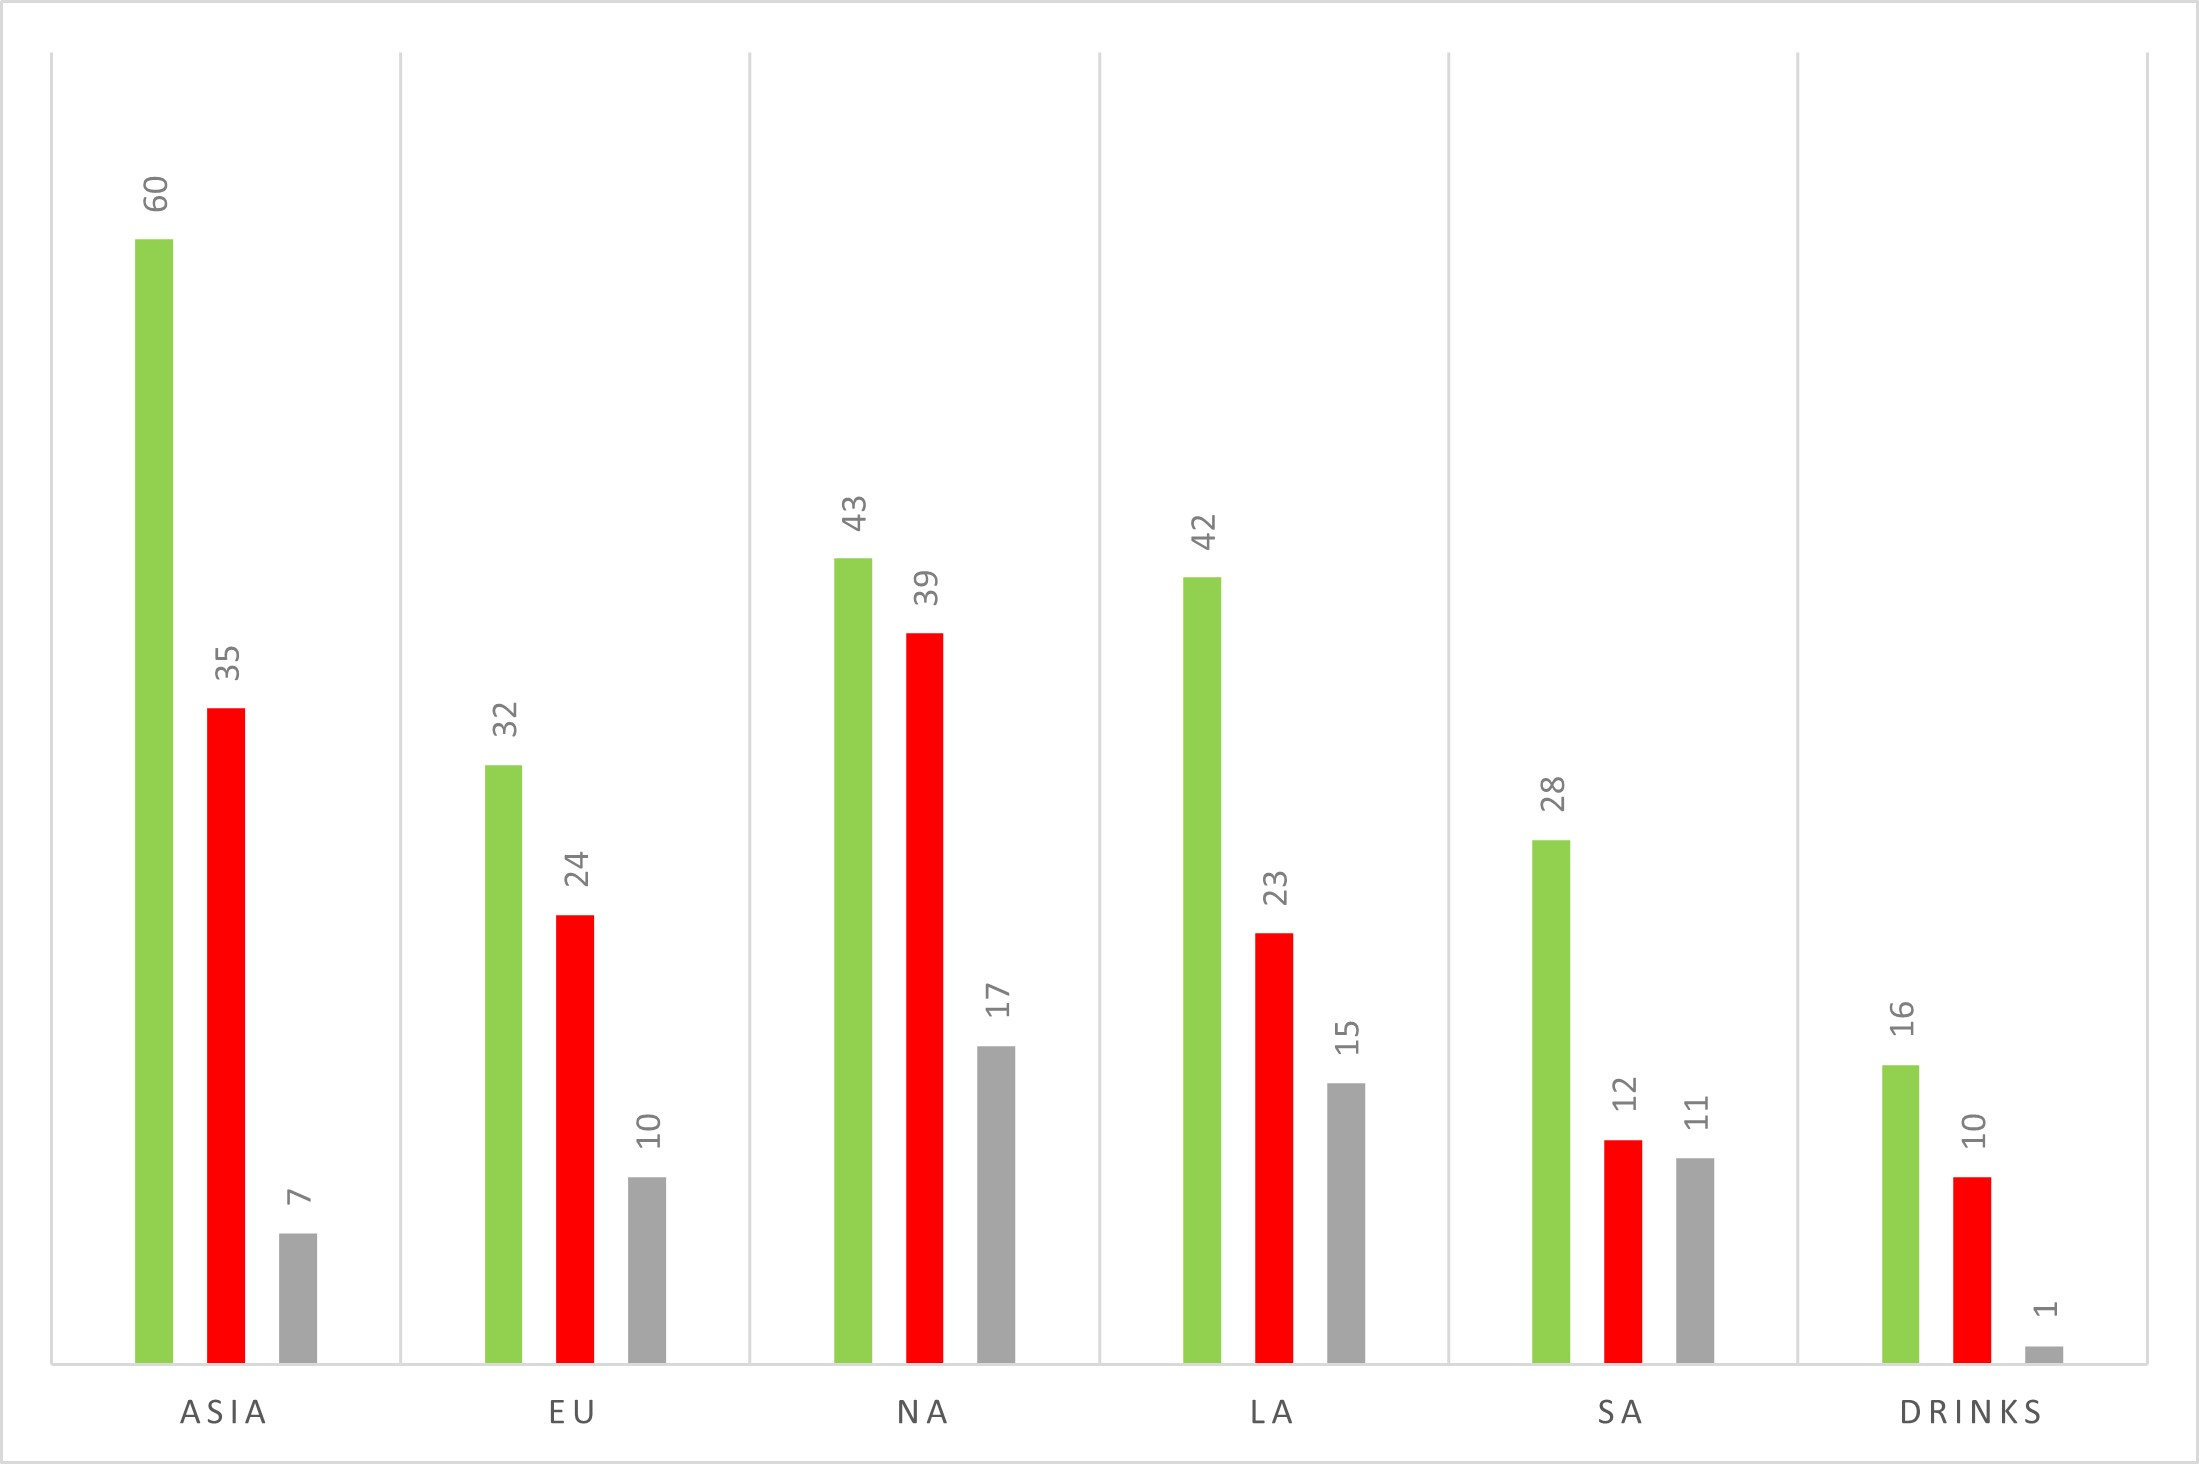
\includegraphics[scale=0.5]{Figures/regions_asela.jpg}
	\caption[Categorization for ingredients from diffrent regions, initial Implementation]{Categorization for ingredients from diffrent regions, initial Implementation}\label{fig:reg_asela}
\end{figure}
\begin{figure}
	\centering
	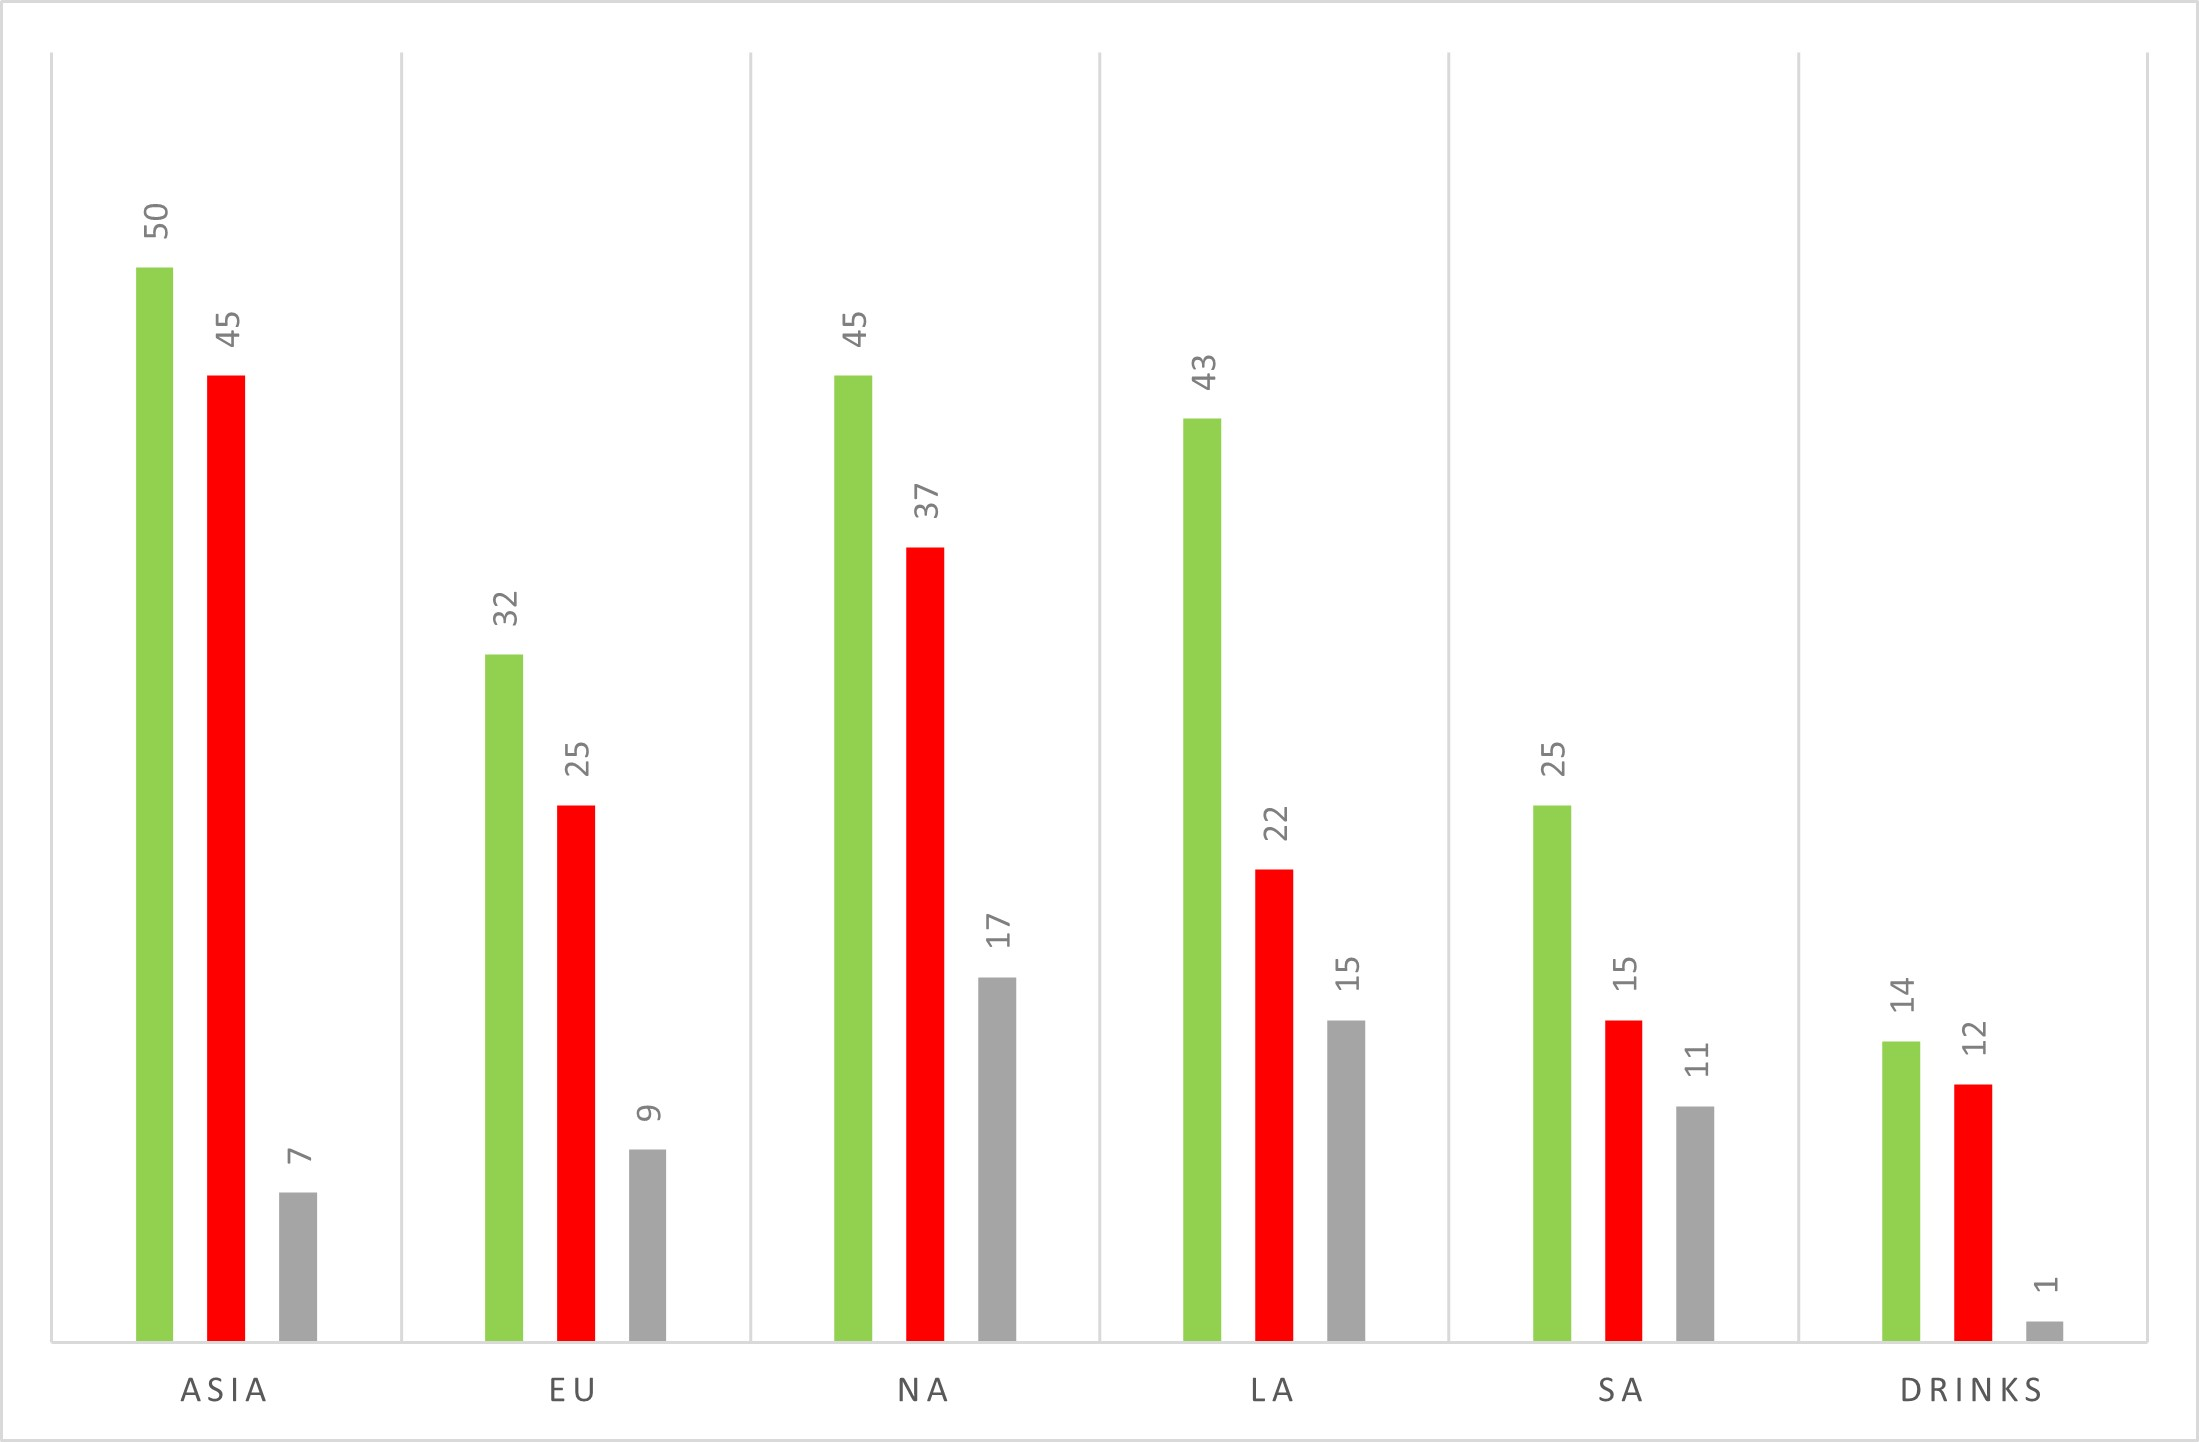
\includegraphics[scale=0.5]{Figures/regions_mm.jpg}
	\caption[Categorization for ingredients from diffrent regions, our Implementation]{Categorization for ingredients from diffrent regions, our Implementation}\label{fig:reg_mm}
\end{figure}

\subsection{Problems with the preprocesser for categorization}\label{sub:problem}
\section{Grocery List Generation}\label{sec:eval_list}


